\documentclass[11pt]{article}

% parameters are fairly self-explanatory here, thankfully
\usepackage[width=7in,height=9.5in,top=0.75in,centering]{geometry}

% for math-ing
\usepackage{amsmath}
\usepackage{amssymb}
\usepackage{enumerate}% http://ctan.org/pkg/enumerate

\usepackage{tasks}
\newcommand{\tasksA}[2]{\begin{tasks}(#1) #2 \end{tasks}} %use alpha labels

%%%%%% tables %%%%%%%%

\usepackage{array}
\renewcommand{\arraystretch}{1.5}
\setlength{\tabcolsep}{8pt}

%%%%%% plotting %%%%%%

\usepackage[dvipsnames]{xcolor}
\usepackage{tikz}
\usepackage{pgfplots}

\pgfplotsset{every axis/.append style={
                    axis x line=middle,    % put the x axis in the middle
                    axis y line=middle,    % put the y axis in the middle
                    axis line style={<->,color=black}, % arrows on the axis
                    xlabel={$x$},          % default put x on x-axis
                    ylabel={$y$},          % default put y on y-axis
            }}
            
 \pgfplotsset{compat=1.14} % sometimes, everything falls apart without this
 
 %\usepgfplotslibrary{fillbetween} %for shading between curves

%%%%%% commands %%%%%%

% exam heading; course name is first argument, exam information is second argument
\newcommand{\Heading}[2]{
    \fbox{
        {\Large\textbf{#1}}
        }
    \hfill
    \fbox{
        \begin{minipage}{0.2\textwidth}
            \begin{center}
            \textbf{#2}
            \end{center}
        \end{minipage}
    }
    \par\vspace{0.1in}}

% for being lazy while beautifying integrals
\newcommand{\dint}{\displaystyle\int}

% for being lazy while beautifying limits
\newcommand{\dlim}{\displaystyle\lim}

%%%%%% stuff %%%%%%

\usepackage{fancyhdr}

%\setcounter{page}{0} % first page is page 0

\parindent0pt % no indent

\fboxsep=0.25cm % little space in fbox border

%%%%%% BEGIN! %%%%%%%

\begin{document}

\pagestyle{fancy}

% record goals here to create sense of transparency

\fancyhead[c]{%
  \ifcase\value{page}
  % empty test for page = 0
  \or {}% 
  \or
  \or {\bf\color{RedOrange} A2: Local and Absolute Extreme Values}% page=1
  \or {\bf\color{RedOrange} A3: Applied Optimization}% page = 2
  \or {\bf\color{Fuchsia} I1: Meaning of an Integral}% page = 3
  \or {\bf\color{Fuchsia} I2: Properties of Definite Integrals}% page = 4
  \or {\bf\color{Fuchsia} I3: Antiderivatives and Indefinite Integrals}% page = 5
  \or {\bf\color{Fuchsia} I4: Compute Definite Integrals}% page = 6
  \or {\bf\color{ProcessBlue} F3: Summations}% page = 7
  \or {\bf\color{Orange} P1: Discrete Random Variables}% page = 8
  \or {\bf\color{Orange} P2: Continuous Random Variables}% page = 9
  \or
  \else
  % Empty chead here!
  \fi
}

\thispagestyle{empty} % don't display that this is page 0

\Heading{MATH 1190/1210 Survey of Calculus I}{Knowledge Checkpoint 4\\Growth-Based\\Fall 2025}

\vspace{0.1in}

\textbf{Name} \hrulefill \, \begin{minipage}{0.16\textwidth}\begin{center}\textbf{UVA ID\\ (e.g. hdj4nd)} \end{center}\end{minipage}\hrulefill\\

\begin{minipage}{0.2\textwidth}\begin{center}\textbf{Course \&\\ Section Number} \end{center}\end{minipage} \hrulefill\,\,\textbf{Date} \hrulefill  \\

\hrulefill
\paragraph*{Course \& Section Numbers:}

{\small
\begin{center}
\begin{tabular}{| c | c | c | c |}
\hline
\begin{minipage}{0.12\textwidth}\centering
1190-100\\
J. Rolf\\
(2:00 PM)
\end{minipage}
&
\begin{minipage}{0.12\textwidth}\centering
1190-200\\
J. Rolf\\
(3:30 PM)
\end{minipage}
&
\begin{minipage}{0.12\textwidth}\centering
1190-300\\
Michael\\
(11 AM)
\end{minipage}
&
\begin{minipage}{0.12\textwidth}\centering
1210-200\\
Susan\\
(9:30 AM)
\end{minipage}
\\ \hline
\begin{minipage}{0.12\textwidth}\centering
1210-300\\
Susan\\
(2 PM)
\end{minipage}
&
\begin{minipage}{0.12\textwidth}\centering
1210-400\\
Holden\\
(12:30 PM)
\end{minipage}
&
\begin{minipage}{0.12\textwidth}\centering
1210-500\\
Susan\\
(3:30 PM)
\end{minipage}
&
\begin{minipage}{0.12\textwidth}\centering
1210-700\\
Aaratrick\\
(2:00 PM)
\end{minipage}
\\ \hline
\begin{minipage}{0.12\textwidth}\centering
1210-800\\
J. Bowling\\
(3:30 PM)
\end{minipage}
&
\begin{minipage}{0.12\textwidth}\centering
1210-900\\
J. Bowling\\
(5 PM)
\end{minipage}
&
\begin{minipage}{0.12\textwidth}\centering
1210-930\\
Vadim\\
(11 AM)
\end{minipage}
\\
\cline{1-3}
\end{tabular}
\end{center}
}

{%\small

\paragraph*{Instructions:}

\begin{itemize}
    
    \item The regular time allowed for completing this assessment is \fbox{$90$} minutes.
    %\item This assessment is out of 50 points.\\
    \item This assessment contains one single-part or multi-part problem for each of the following targets:  {\bf\color{RedOrange}A2}, {\bf\color{RedOrange}A3}, {\bf\color{Fuchsia}I1}, {\bf\color{Fuchsia}I2}, {\bf\color{Fuchsia}I3}, {\bf\color{Fuchsia}I4}, {\bf\color{ProcessBlue}F3}, {\bf\color{Orange}P1}, {\bf\color{Orange}P2}.
    \item On each problem, you will receive a score of Exceeds Expectations (5), Proficient (4), Almost (3), Developing (2), Emerging (1), or Not Yet (0). {\bf Please do not interpret your score as a percentage.}
    %\item You will have opportunities to reassess on the targets appearing on this assessment after the next {\bf 2} assessments.\\
    \item You may NOT use calculators, dictionaries, notes, phones, or any other kind of aid.
    \item Please write neatly. What cannot be read, cannot be graded.
    \item Carefully work out each problem and clearly indicate your final answer to every problem.
    \item Throughout, give the most descriptive answer possible. \textbf{For instance, ``DNE" will not be accepted when ``$=\infty$" is applicable.}
    %\item Please provide the most specific answer possible. For instance, if a limit does not exist because it goes to $\infty$ or $-\infty$, then specify this.
    \item Please use the methods discussed up to this point in the course. For example, any work based on l'H\^opital's Rule will not receive credit.
    \item \textbf{All work must be shown unless otherwise specified.} Partial credit will not be given if appropriate work is not shown.
    \item In particular, {\bf any answer appearing with no justification will receive no credit regardless of whether the answer was correct}, unless otherwise specified.
    \item Please first respond to the prompts on which you feel most proficient, then respond to others later.
    \item This booklet is printed double-sided. It contains 14 pages and 9 numbered problems.
    \item There's a formula sheet on the second-to-last page of common area/volume formulas and optimization concepts in case you need them.
    \end{itemize}
    
    }

\vfill


%%%%%%%%%
\newpage

This page is left blank intentionally.\\

Use this page if you need additional space to write your solutions to any problem. \\

If you wish this page graded, you must refer to this page on \textbf{the original page} of the problem. Otherwise, your grader will NOT consider your work on this page.

\newpage%
%%%%%%%%%


\begin{enumerate}

%%%%%%%%%%%%%%%%%%%%%%%%%%%%%%%%%%%%%%%%%%%%%%%%%%%%%
%%%%%%%%%%% BEGIN PROBLEM A2 %%%%%%%%%%%%%%%%%%%%%%%%
%%%%%%%%%%%%%%%%%%%%%%%%%%%%%%%%%%%%%%%%%%%%%%%%%%%%%

\item Consider the following function $f(x)$.

\[f(x)=x^2 - x\]%-(x-1)^4(15x^2+18x+7)\]

%\[f'(x)=15x^2(x-1)(x+1)\]%10(1-x)^3(3x+1)^2\]

You are required to use methods we've learned in our course, such as the first derivative test, the second derivative test, the close interval method, or the first derivative test for absolute extrema, to solve this problem. In addition, you need to make sure the method you use is suitable for the question.

\begin{enumerate}
    \item Find all critical numbers of $f(x)$.

    \vfill

    \item For each critical number found in part (a), classify it as a local minimum, a local maximum, or neither. Fully justify your work.

    \vfill
    \vfill
    \vfill

    \item Find the $x$-values of all absolute extrema of $f(x)$ on the interval $[-2, 2]$.

    \vfill
    \vfill
    \vfill
\end{enumerate}

%%%%%%%%%%%%%%%%%%%%%%%%%%%%%%%%%%%%%%%%%%%%%%%%%%%%%
%%%%%%%%%%% END PROBLEM A2 %%%%%%%%%%%%%%%%%%%%%%%%%%
%%%%%%%%%%%%%%%%%%%%%%%%%%%%%%%%%%%%%%%%%%%%%%%%%%%%%

\newpage

%%%%%%%%%%%%%%%%%%%%%%%%%%%%%%%%%%%%%%%%%%%%%%%%%%%%%
%%%%%%%%%%% BEGIN PROBLEM A3 %%%%%%%%%%%%%%%%%%%%%%%%
%%%%%%%%%%%%%%%%%%%%%%%%%%%%%%%%%%%%%%%%%%%%%%%%%%%%%

\item A rectangular garden is to be constructed using a river as one side of the garden and wire fencing for the other three sides. Given 100 ft of wire fencing, determine the dimensions that would create a garden of maximum area. What is the maximum area?
\vspace{0.5cm}

% \begin{figure}[h]
%     \centering
%     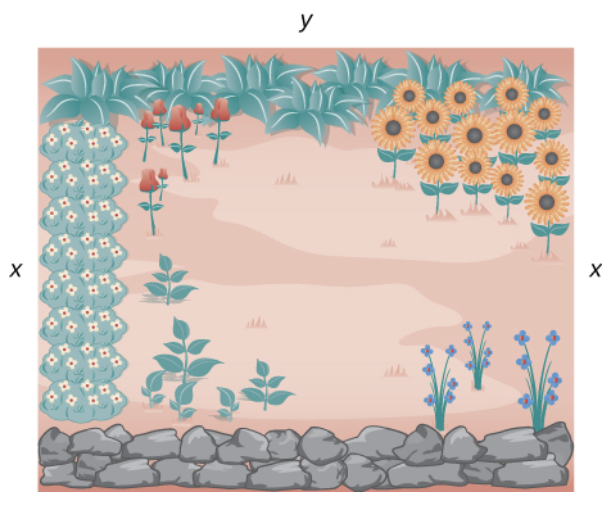
\includegraphics[width=0.5\textwidth]{Garden.png}
%     \caption{Rectangular garden with one side along a rock wall}
%     \label{fig:garden}
% \end{figure}
\begin{tikzpicture}[scale=0.08]

% River (top side, no fence)
\draw[thick, blue] (0,50) -- (120,50);
\node[blue, above] at (60,50) {River (no fence)};

% Rectangle (garden)
\draw[thick] (0,0) rectangle (120,50);

% Labels for sides
\node at (60,-5) {$x$ ft};
\node at (-8,30) {$y$ ft};
\node at (128,30) {$y$ ft};

% Fence labels
\node at (60,55) {}; % no fence on river
\node at (60,-12) {Fence};
\node at (-12,25) {Fence};
\node at (135,25) {Fence};

% Corner points (optional)
\fill (0,0) circle (2);
\fill (120,0) circle (2);
\fill (0,50) circle (2);
\fill (120,50) circle (2);

\end{tikzpicture}




To receive full credit, make sure to clearly state:

\begin{itemize}
    \item The function you wish to maximize\\
    \item A domain/interval for optimization\\
    \item The dimensions that maximize the area\\
    \item The maximium area\\
    \item A mathematical justification that this is the maximum area.
\end{itemize}


%%%%%%%%%%%%%%%%%%%%%%%%%%%%%%%%%%%%%%%%%%%%%%%%%%%%%
%%%%%%%%%%% END PROBLEM A3 %%%%%%%%%%%%%%%%%%%%%%%%%%
%%%%%%%%%%%%%%%%%%%%%%%%%%%%%%%%%%%%%%%%%%%%%%%%%%%%%

\newpage

%%%%%%%%%%%%%%%%%%%%%%%%%%%%%%%%%%%%%%%%%%%%%%%%%%%%%
%%%%%%%%%%% BEGIN PROBLEM I1 %%%%%%%%%%%%%%%%%%%%%%%%
%%%%%%%%%%%%%%%%%%%%%%%%%%%%%%%%%%%%%%%%%%%%%%%%%%%%%
\item Let $r'(t)$ represent the rate of water consumed by a data center, in gallons per hour ($\text{gal/hr}$), where $t$ is the number of hours since midnight. (\textbf{Note:} Here 12:00am = 0, 1:00am = 1, etc.)
    


    \begin{enumerate}[i]
        \item What are the units of $\displaystyle\int_0^8 r'(t) \, dt$?
        \vspace{6cm}

        \item Explain the meaning of $\displaystyle\int_0^8 r'(t) \, dt$ in this context.
       \vspace{6cm}

%        \item Is $\displaystyle \int_0^{24} r'(t)\,dt$ positive, negative, or zero?
       % \vspace{1cm}

       %  \begin{itemize}
       %      \item[$\square$] Positive
       %      \item[$\square$] Negative
       %      \item[$\square$] Zero
       %  \end{itemize}
       %         \vspace{3cm}

    \item If $r(a)=5$, express $r(b)$ in terms of $r(a)$ and $\displaystyle \int_a^b r'(t)\,dt$.
\end{enumerate}


%%%%%%%%%%%%%%%%%%%%%%%%%%%%%%%%%%%%%%%%%%%%%%%%%%%%%
%%%%%%%%%%% END PROBLEM I1 %%%%%%%%%%%%%%%%%%%%%%%%%%
%%%%%%%%%%%%%%%%%%%%%%%%%%%%%%%%%%%%%%%%%%%%%%%%%%%%%

\newpage

%%%%%%%%%%%%%%%%%%%%%%%%%%%%%%%%%%%%%%%%%%%%%%%%%%%%%
%%%%%%%%%%% BEGIN PROBLEM I2 %%%%%%%%%%%%%%%%%%%%%%%%
%%%%%%%%%%%%%%%%%%%%%%%%%%%%%%%%%%%%%%%%%%%%%%%%%%%%%

\item Suppose the following values of definite integrals are given.

\[
\int_{0}^{3} g(x)\,dx = 5
\quad
\int_{-2}^{0} g(x)\,dx = -2
\quad
\int_{3}^{0} 2(f(x) - g(x))\,dx = 10
\quad
\int_{-2}^{3} (f(x) - g(x))\,dx = 6
\]

Find the value of the following definite integrals.

\tasksA{2}{
\task $\displaystyle \int_{3}^{3} g(x)\, dx$

\task $\displaystyle \int_{0}^{3} f(x)\, dx$

\vspace{7cm}

\task $\displaystyle \int_{-2}^{3} f(x)\, dx$
}
%%%%%%%%%%%%%%%%%%%%%%%%%%%%%%%%%%%%%%%%%%%%%%%%%%%%%
%%%%%%%%%%% END PROBLEM I2 %%%%%%%%%%%%%%%%%%%%%%%%%%
%%%%%%%%%%%%%%%%%%%%%%%%%%%%%%%%%%%%%%%%%%%%%%%%%%%%%

\newpage

%%%%%%%%%%%%%%%%%%%%%%%%%%%%%%%%%%%%%%%%%%%%%%%%%%%%%
%%%%%%%%%%% BEGIN PROBLEM I3 %%%%%%%%%%%%%%%%%%%%%%%%
%%%%%%%%%%%%%%%%%%%%%%%%%%%%%%%%%%%%%%%%%%%%%%%%%%%%%

\item Assume $x>0$. Write down the indefinite integrals of the following expressions. 

Although no work is required, you are encouraged to include any work that shows your thought process. 

%constant, power, exponential, log, +C, algebraic manipulation

\begin{center}
        \begin{tabular}{l c r l c r}
            %
            $\displaystyle\int 3\,dx$ & $=$ & \rule[-8pt]{1.5in}{0.4pt} &
                \vspace{5cm}

            %
            %$\displaystyle\int \,dx$ & $=$ & \rule[-8pt]{1.5in}{0.4pt}\\[0.3in]
            %%%%%
            %$\displaystyle\int 15\,dx$ & $=$ & \rule[-8pt]{1.5in}{0.4pt} & 
            %%%%%
            $\displaystyle\int \dfrac{1}{x^7} \,dx$ & $=$ & \rule[-8pt]{1.5in}{0.4pt}\\[1in]
                \vspace{5cm}

            %%%%%
            $\displaystyle\int 3^x\,dx$ & $=$ & \rule[-8pt]{1.5in}{0.4pt}&
            %
            $\displaystyle\int x^3 + 2x\,dx$ & $=$ & \rule[-8pt]{1.5in}{0.4pt}\\[1in]
            %%%%%
            $\displaystyle\int 3x^4 \,dx$ & $=$ & \rule[-8pt]{1.5in}{0.4pt} & 
            %
            $\displaystyle\int \dfrac{1}{x} \,dx$ & $=$ & \rule[-8pt]{1.5in}{0.4pt}\\[0.3in]
            %%%%%
        \end{tabular}
\end{center}

%%%%%%%%%%%%%%%%%%%%%%%%%%%%%%%%%%%%%%%%%%%%%%%%%%%%%
%%%%%%%%%%% END PROBLEM I3 %%%%%%%%%%%%%%%%%%%%%%%%%%
%%%%%%%%%%%%%%%%%%%%%%%%%%%%%%%%%%%%%%%%%%%%%%%%%%%%%

\newpage

%%%%%%%%%%%%%%%%%%%%%%%%%%%%%%%%%%%%%%%%%%%%%%%%%%%%%
%%%%%%%%%%% BEGIN PROBLEM I4 %%%%%%%%%%%%%%%%%%%%%%%%
%%%%%%%%%%%%%%%%%%%%%%%%%%%%%%%%%%%%%%%%%%%%%%%%%%%%%

\item For each of the following definite integrals, determine whether the Fundamental Theorem of Calculus can be applied to evaluate. 

If so, evaluate the integral using the FTC. There's no need to simplify your final answer.

If not, clearly explain why.

\begin{enumerate}
    \item $\displaystyle\int_{0}^{2}\dfrac{1}{x-1}\, dx$

    \vfill

    \item $\displaystyle\int_{0}^1  \frac{x^2}{2}+ \frac{5}{6}\, dx$

    \vfill

%    \item $\displaystyle\int_{-3}^1\dfrac{1}{x^2}- \frac{x^2}{2}\, dx$

%    \vfill
   \item $\displaystyle\int_{1}^2\dfrac{1}{x}- \frac{x}{2}\, dx$

    \vfill
\end{enumerate}

%%%%%%%%%%%%%%%%%%%%%%%%%%%%%%%%%%%%%%%%%%%%%%%%%%%%%
%%%%%%%%%%% END PROBLEM I4 %%%%%%%%%%%%%%%%%%%%%%%%%%
%%%%%%%%%%%%%%%%%%%%%%%%%%%%%%%%%%%%%%%%%%%%%%%%%%%%%

\newpage

%%%%%%%%%%%%%%%%%%%%%%%%%%%%%%%%%%%%%%%%%%%%%%%%%%%%%
%%%%%%%%%%% BEGIN PROBLEM F3 %%%%%%%%%%%%%%%%%%%%%%%%
%%%%%%%%%%%%%%%%%%%%%%%%%%%%%%%%%%%%%%%%%%%%%%%%%%%%%

\item 

\begin{enumerate}
    \item Find the value of the following expressions. Simplify as much as possible so that your final answer is a number.

    \begin{enumerate}
        \item[(i)] $\displaystyle\sum_{i=4}^5 3$

        \vfill

        \item[(ii)] $\displaystyle\sum_{j=2}^4(j-j^2)$

        \vfill
    \end{enumerate}

    \item Write the following sum in summation notation. 

    \[\dfrac{1}{1}-\dfrac{1}{2}+\dfrac{1}{4}-\dfrac{1}{8}\]

    \vfill
\end{enumerate}

%%%%%%%%%%%%%%%%%%%%%%%%%%%%%%%%%%%%%%%%%%%%%%%%%%%%%
%%%%%%%%%%% END PROBLEM F3 %%%%%%%%%%%%%%%%%%%%%%%%%%
%%%%%%%%%%%%%%%%%%%%%%%%%%%%%%%%%%%%%%%%%%%%%%%%%%%%%

\newpage

%%%%%%%%%%%%%%%%%%%%%%%%%%%%%%%%%%%%%%%%%%%%%%%%%%%%%
%%%%%%%%%%% BEGIN PROBLEM P1 %%%%%%%%%%%%%%%%%%%%%%%%
%%%%%%%%%%%%%%%%%%%%%%%%%%%%%%%%%%%%%%%%%%%%%%%%%%%%%

\item Let $X$ be a discrete random variable, and let $p(x)$ be its probability mass function.

\begin{enumerate}
    \item Consider the following table. Fill in the missing value to make the table into a valid probability mass function. 

    \vspace{0.5cm}

    \begin{minipage}{0.45\textwidth}
        \centering    
        \begin{tabular}{c|ccc}
            \hline
           $x$  & 1 & 2 & 3  \\
           \hline
           $p(x)$  & 0.25 &  & 0.25\\
           \hline
        \end{tabular}
    \end{minipage}


   \vspace{1cm}
%    \item Find $P(X\text{ is odd})$.
 %   \vspace{3cm}


  \item Calculate the expectation $E[X]$ of $X$.
    \vspace{6cm}

\item Histograms representing the PMFs of random variables $X_1$, $X_2$, and $X_3$ (respectively) are given below. Without computing the variances explicitly, rank the random variables from smallest variance to largest variance. Briefly justify your answer.

\begin{center}
\begin{tabular}{ c c c }

%---------------- X1 ----------------
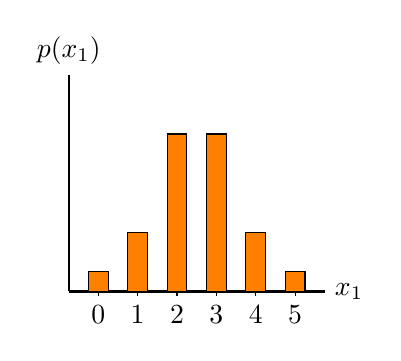
\begin{tikzpicture}[scale=0.25]
% axes
\draw[thick](0,0)--(0,11) node[above]{$p(x_1)$};
\draw[thick](0,0)--(13,0) node[right]{$x_1$};

% x labels
\foreach \x/\lab in {1.5/0,3.5/1,5.5/2,7.5/3,9.5/4,11.5/5}
\draw (\x,0.25)--(\x,-0.25) node[below]{$\lab$};

% histogram (very concentrated around middle)
\draw[fill=orange] (1,0)--(2,0)--(2,1)--(1,1)--cycle;
\draw[fill=orange] (3,0)--(4,0)--(4,3)--(3,3)--cycle;
\draw[fill=orange] (5,0)--(6,0)--(6,8)--(5,8)--cycle;
\draw[fill=orange] (7,0)--(8,0)--(8,8)--(7,8)--cycle;
\draw[fill=orange] (9,0)--(10,0)--(10,3)--(9,3)--cycle;
\draw[fill=orange] (11,0)--(12,0)--(12,1)--(11,1)--cycle;
\end{tikzpicture}

&

%---------------- X2 ----------------
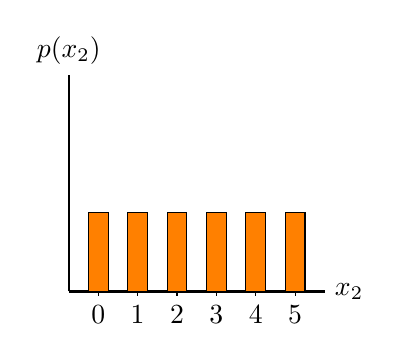
\begin{tikzpicture}[scale=0.25]
% axes
\draw[thick](0,0)--(0,11) node[above]{$p(x_2)$};
\draw[thick](0,0)--(13,0) node[right]{$x_2$};

% x labels
\foreach \x/\lab in {1.5/0,3.5/1,5.5/2,7.5/3,9.5/4,11.5/5}
\draw (\x,0.25)--(\x,-0.25) node[below]{$\lab$};

% histogram (roughly uniform)
\draw[fill=orange] (1,0)--(2,0)--(2,4)--(1,4)--cycle;
\draw[fill=orange] (3,0)--(4,0)--(4,4)--(3,4)--cycle;
\draw[fill=orange] (5,0)--(6,0)--(6,4)--(5,4)--cycle;
\draw[fill=orange] (7,0)--(8,0)--(8,4)--(7,4)--cycle;
\draw[fill=orange] (9,0)--(10,0)--(10,4)--(9,4)--cycle;
\draw[fill=orange] (11,0)--(12,0)--(12,4)--(11,4)--cycle;
\end{tikzpicture}

&

%---------------- X3 ----------------
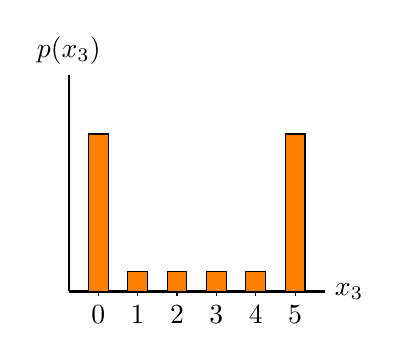
\begin{tikzpicture}[scale=0.25]
% axes
\draw[thick](0,0)--(0,11) node[above]{$p(x_3)$};
\draw[thick](0,0)--(13,0) node[right]{$x_3$};

% x labels
\foreach \x/\lab in {1.5/0,3.5/1,5.5/2,7.5/3,9.5/4,11.5/5}
\draw (\x,0.25)--(\x,-0.25) node[below]{$\lab$};

% histogram (mass at extremes)
\draw[fill=orange] (1,0)--(2,0)--(2,8)--(1,8)--cycle;
\draw[fill=orange] (3,0)--(4,0)--(4,1)--(3,1)--cycle;
\draw[fill=orange] (5,0)--(6,0)--(6,1)--(5,1)--cycle;
\draw[fill=orange] (7,0)--(8,0)--(8,1)--(7,1)--cycle;
\draw[fill=orange] (9,0)--(10,0)--(10,1)--(9,1)--cycle;
\draw[fill=orange] (11,0)--(12,0)--(12,8)--(11,8)--cycle;
\end{tikzpicture}

\end{tabular}
\end{center}















%%%%%%%%%%%%%%%%%%%%%%%%%%%%%%%%%%%%%%%%%%%%%%%%%%%%%
%%%%%%%%%%% END PROBLEM P1 %%%%%%%%%%%%%%%%%%%%%%%%%%
%%%%%%%%%%%%%%%%%%%%%%%%%%%%%%%%%%%%%%%%%%%%%%%%%%%%%

\newpage

%%%%%%%%%%%%%%%%%%%%%%%%%%%%%%%%%%%%%%%%%%%%%%%%%%%%%
%%%%%%%%%%% BEGIN PROBLEM P2 %%%%%%%%%%%%%%%%%%%%%%%%
%%%%%%%%%%%%%%%%%%%%%%%%%%%%%%%%%%%%%%%%%%%%%%%%%%%%%

\item The lifetime, $X$, in tens of hours, of a battery has (potential) probability density function $p(x)$ given by
\[
p(x) =
\begin{cases}
0, & x < 1, \\
c(x - 1), & 1 \le x \le 3, \\
0, & x > 3.
\end{cases}
\]
\bigskip

\begin{enumerate}[i]
\item Find the value of $c$ that will make $p(x)$ into a valid probability density function.
\vspace{4cm}

\item What is the support of $X$?
\bigskip

$\mathrm{Supp}_{X}$ = \rule[-8pt]{1.5in}{0.4pt}
\bigskip

\item Find $P(2 \le X \le 3)$. 
\vspace{2in}

\item Write down an expression for expectation $E[X]$ of $X$ (You do not need to perform any calculations).
\end{enumerate}



%%%%%%%%%%%%%%%%%%%%%%%%%%%%%%%%%%%%%%%%%%%%%%%%%%%%%
%%%%%%%%%%% END PROBLEM P2 %%%%%%%%%%%%%%%%%%%%%%%%%%
%%%%%%%%%%%%%%%%%%%%%%%%%%%%%%%%%%%%%%%%%%%%%%%%%%%%%

\newpage

\begin{center}
{\bf DO NOT REMOVE THIS SHEET FROM YOUR EXAM PACKET}
\end{center}

\begin{center}
    \begin{tabular}{ r | c | l }
    {\bf Description} & {\bf Formula} & {\bf Variables}\\
    \hline
    area of a square & $A=s^2$ & $s=$ side length\\
    \hline
    area of a rectangle & $A=lw$ & $l=$ length, $w=$ width\\
    \hline
    area of a triangle & $A=\frac12bh$ & $b=$ base, $h=$ height\\
    \hline
    area of a circle & $A=\pi r^2$ & $r=$ radius\\
    \hline
    volume of a rectangular box & $V=lwh$ & $l=$ length, $w=$ width, $h=$ height\\
    \hline
    %volume of a circular cylinder & $V=\pi r^2 h$ & $r=$ radius, $h=$ height\\
    %\hline
    %volume of a sphere & $V=\frac43\pi r^3$ & $r=$ radius\\
    %\hline
    revenue & $R(x) = p\cdot x = p\cdot Q$ & $p=$ unit price, $x=Q=$ quantity sold\\
    \hline
    profit & $P(x) = R(x) - C(x)$ & $R(x)=$ revenue, $C(x)=$ cost\\
    \hline
    average cost & $\overline C(x) = \frac{C(x)}{x}$ & $C(x)=$ cost\\
    \end{tabular}
\end{center}

\begin{center}
{\bf DO NOT REMOVE THIS SHEET FROM YOUR EXAM PACKET}
\end{center}

\newpage

This page is left blank intentionally.\\

Use this page if you need additional space to write your solutions to any problem. \\

If you wish this page graded, you must refer to this page on \textbf{the original page} of the problem. Otherwise, your grader will NOT consider your work on this page.

\newpage

This page is left blank intentionally.\\

Use this page if you need additional space to write your solutions to any problem. \\

If you wish this page graded, you must refer to this page on \textbf{the original page} of the problem. Otherwise, your grader will NOT consider your work on this page.


\end{enumerate}

\end{document}